%\documentclass[handout]{beamer}
\documentclass[•]{beamer}
\usepackage[latin1]{inputenc}
\usepackage{amsmath}



\usetheme{Luebeck}
\setbeamertemplate{footline}[frame number]
\setbeamertemplate{navigation symbols}{}

\newtheorem{proposition}{Proposition}
\newtheorem{exercise}{Exercise}
\theoremstyle{remark}
\newtheorem{remark}[theorem]{Remark}

\mathchardef\sa="303A
\newcommand{\esup}{\mathop{{\rm ess\,sup}}\limits}
\let\Eqnarray=\eqnarray
\renewcommand{\eqnarray}{\arraycolsep=0.1675em \Eqnarray}

\newcommand{\lag}{\mathcal{L}}
\newcommand{\e}{\mathrm{e}}

% enumabc
%
\makeatletter
\newcommand{\enumabc}
	{\expandafter\def\csname the\@enumctr \endcsname{\alph{\@enumctr}}%
	 \expandafter\def\csname label\@enumctr \endcsname
		{\rm(\csname the\@enumctr \endcsname)}}%
\newcommand{\enuminc}[1]{\addtocounter{\@enumctr}{#1}}
\makeatother
%
\subtitle{Transmission properties in a short biased quantum wire}
\title{TFYA17 Project}
\author{Patrik Hallsj\"{o}, Felix Faber}
\date{}
\AtBeginSection[]
{
  \begin{frame}
    \frametitle{Table of Contents}
    \tableofcontents[currentsection]
  \end{frame}
}
\AtBeginSubsection[]
{
  \begin{frame}
    \frametitle{Table of Contents}
    \tableofcontents[currentsection,currentsubsection]
  \end{frame}
}

\begin{document}
\begin{frame}
\titlepage
\end{frame}
\begin{frame}
\tableofcontents
\end{frame}
\section{Introduction}
\begin{frame}[shrink=10]\frametitle{Introduction}
\begin{block}

\begin{itemize}
\item This project was dedicated to study an electron transport in a biased quantum wire.
\item The goals were to construct a solver for the potential and to calculate the transmission and reflection coefficients for an electron sent towards the potential.
\end{itemize}
\end{block}
\end{frame}

\begin{frame}
\begin{block}

The potential used in this presentation:
\begin{eqnarray*}
\label{potential}
V(x) = \beta e V_{sd}+V_{g}tanh(s(x-\Delta x_{1}))\\
-(V_{sd}+V_{g})tanh(s(x-\Delta x_{2}))
\end{eqnarray*}
\end{block}
\begin{remark}
\begin{itemize}
\item $\beta=$ Potential drop, if 0.5 then symmetric as in our case.
\item $V_{sd} =$ Bias voltage.
\item $V_g =$ Potential height
\item $S=$ Potential steepness.
\end{itemize}
\end{remark}
\end{frame}
\begin{frame}\frametitle{Goals}
\begin{block}

\begin{itemize}
\item To set and to solve a problem with boundary conditions when an electron is injected into a wire.
\pause
\item To calculate the transmission and reflection coefficients as functions of energy of injected electron and bias.
\pause
\item To represent solutions in graphical form.
\pause
\item Optional: to calculate a conductance.
\end{itemize}
\end{block}
\pause
\begin{remark}
Matlab was used to achieve the goals.
\end{remark}
\end{frame}
\section{Theory}

\begin{frame}\frametitle{Finite derivatives}
\begin{block}

\begin{itemize}
\item $f'(x) =\frac{f(x+h)-f(x+k)}{h-k}$
\pause
\item Forward: $\frac{f(x+h)-f(x)}{h}$
\pause
\item Backward: $\frac{f(x)-f(x-k)}{k}$
\pause
\item Central: $\frac{f(x-h/2)-f(x+h/2)}{h}$
\pause
\item Second order: $\frac{f(x-h)- 2f(x) +f(x+h)}{h^2}$
\end{itemize}
\end{block}
\end{frame}

\begin{frame}\frametitle{Finite steps in differential equations}
\begin{block}

Solve the stationary Schr\"odinger equation which is a second order differential equation:\pause
$ E \psi (x) = (\frac{-\hbar ^2}{2m^*} \frac{\partial}{\partial x} +V(x)) \psi (x)$
\pause
\begin{itemize}
\item Second order differential equation without any first order terms $y''(x) = g(y(x),x)$
\pause
\item Boundary conditions: $y(x_{0}) = y_{0}$ and $y(x_{N}) = y_{N}$, on the interval $[x_{0},x_{N}]$ where$ d = (\frac{x_{o}-x_{N}}{N})$.
\pause
\item $h = d$ and $x = nd$  yields $dg(y(nd),nd) + 2y(nd)-(y((n+1)d)+y((n-1)d)) = 0$.

\item  $N+1$ equations with $N+1$ unknowns.
\end{itemize}
\end{block}
\end{frame}

\begin{frame}\frametitle{Quantum barrier problem}
\begin{block}

Solve the stationary Schr\"odinger equation. With $k=\sqrt{\frac{2m^*}{hbar^2}(E-\beta e V_{Sd})}$ and $k'=\sqrt{\frac{2m^*}{hbar^2}(E+ (1-\beta) e V_{Sd})}$ 
\pause
\begin{itemize}
\item Boundary conditions: $y_{0} = I\exp{(-i k x_{0})} + r\exp{(i k x_{0})}$ and $y_{N} = t\exp{(-i k' x_{N})}$
\pause
\item We have put $I=1$, which gives $y_{0} = \exp{(-i k x_{0})} + r\exp{(i k x_{0})}$ to make the equations easier to solve.
\pause
\item $R$ and $T$ give $N+3$ unknowns but only $N+1$ equations. 
\pause
\item Continuous at boundaries yeilding: $N+3$ unknowns and $N+3$ equations which will have a unique solution.
\end{itemize}
\end{block}
\end{frame}

\section{Results}
\begin{frame}\frametitle{Numerical values}
\begin{block}

The program produces the following data, as well as images of the wave-functions and the potential barriers.
\begin{eqnarray*}
R=|r|^2/(|r|^2+|t|^2)\\
T=|t|^2/(|r|^2+|t|^2)\\
C \propto T/(R+T)
\end{eqnarray*}
\end{block}
\end{frame}

\begin{frame}
\begin{figure}
\centering
\caption{Amplitudes of wave-functions (upper graph) and potential barriers (lower graph) for the case: E=1, $\beta=0.5$, $x_1=4$, $x_2=6$, $V_{sd}=0.3$, $V_g=0.6$}
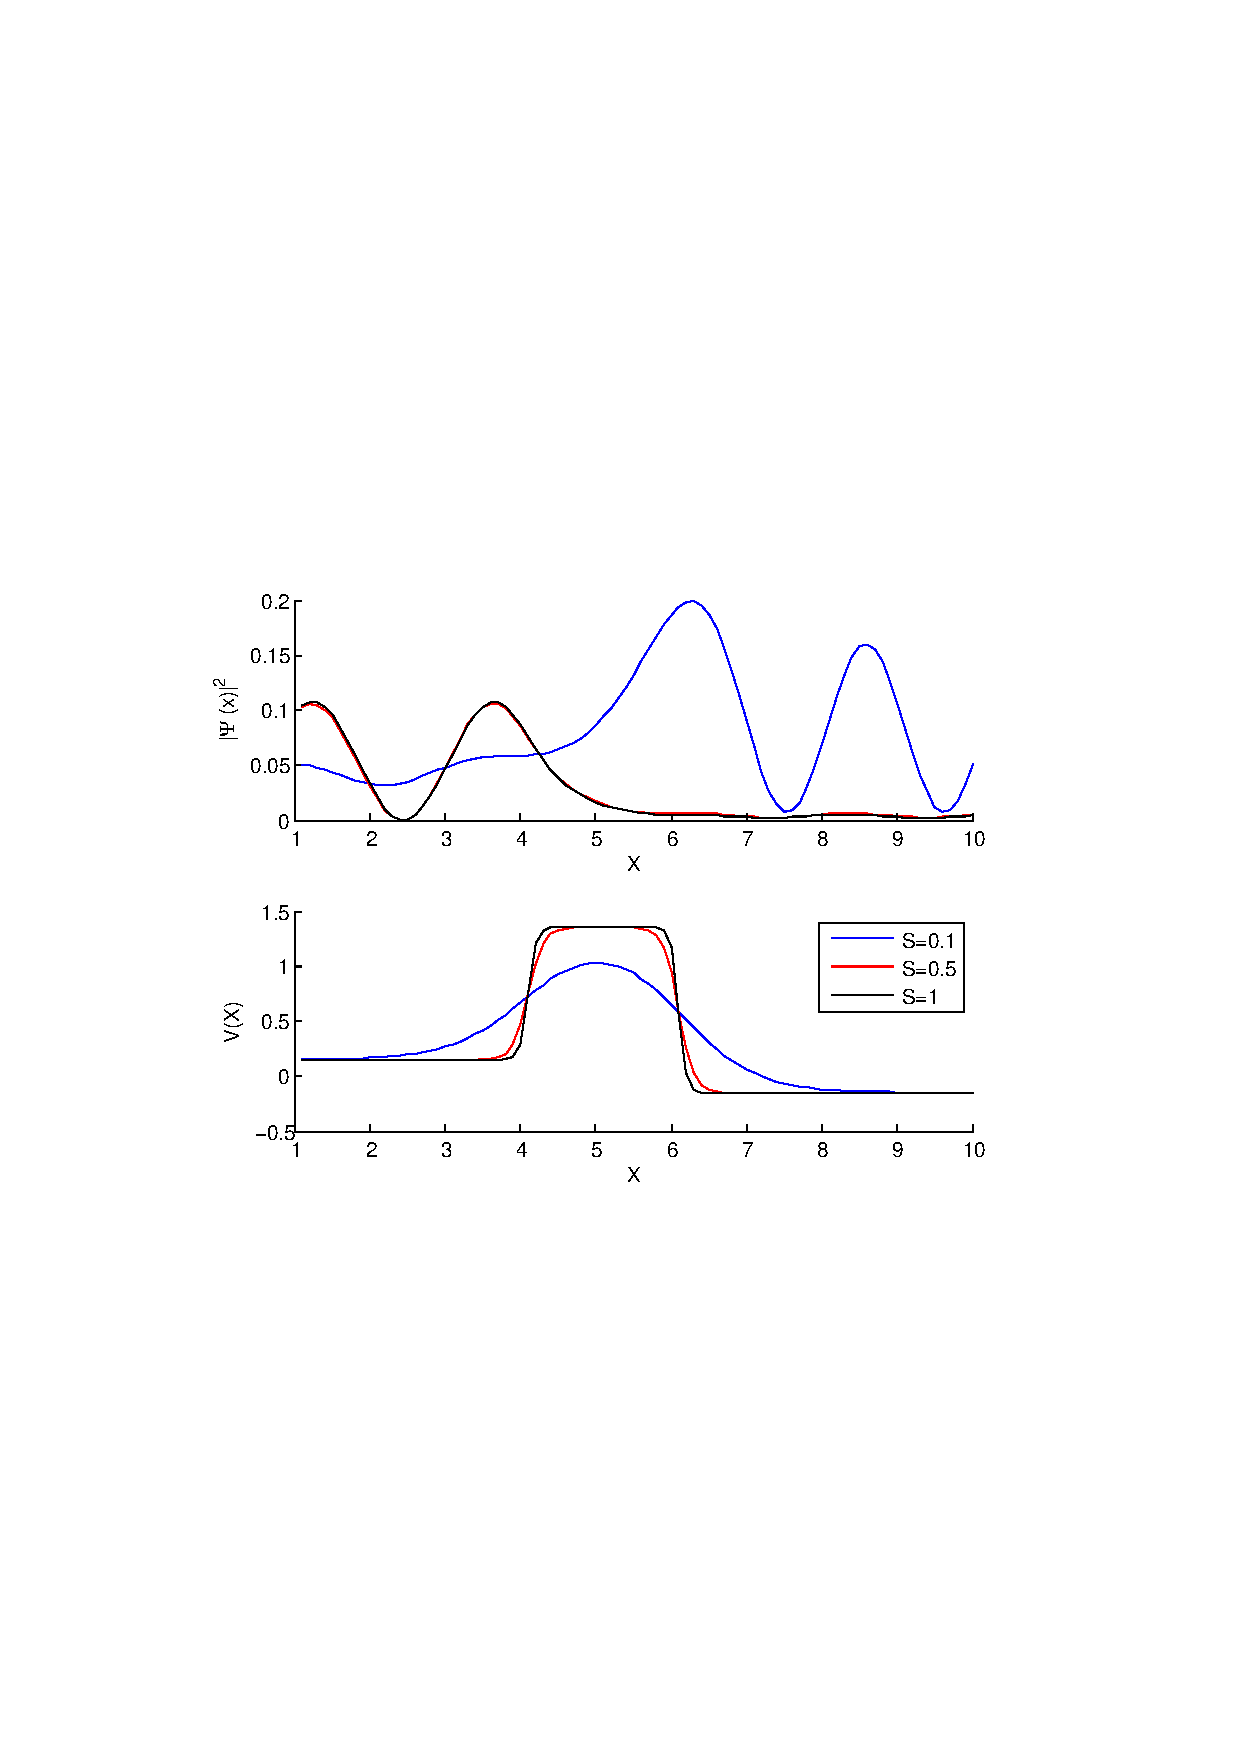
\includegraphics[scale=0.4, trim = 0mm 20mm 0mm 60mm, clip]{test}
\label{fig:test}
\end{figure}
\end{frame}

\begin{frame}
\begin{figure}
\centering
\caption{Amplitudes of wave-functions (upper graph) and potential barriers (lower graph) for the case: E=1, $\beta=0.5$, $x_1=4$, $x_2=6$, $V_{sd}=0.6$, $V_g=0.3$}
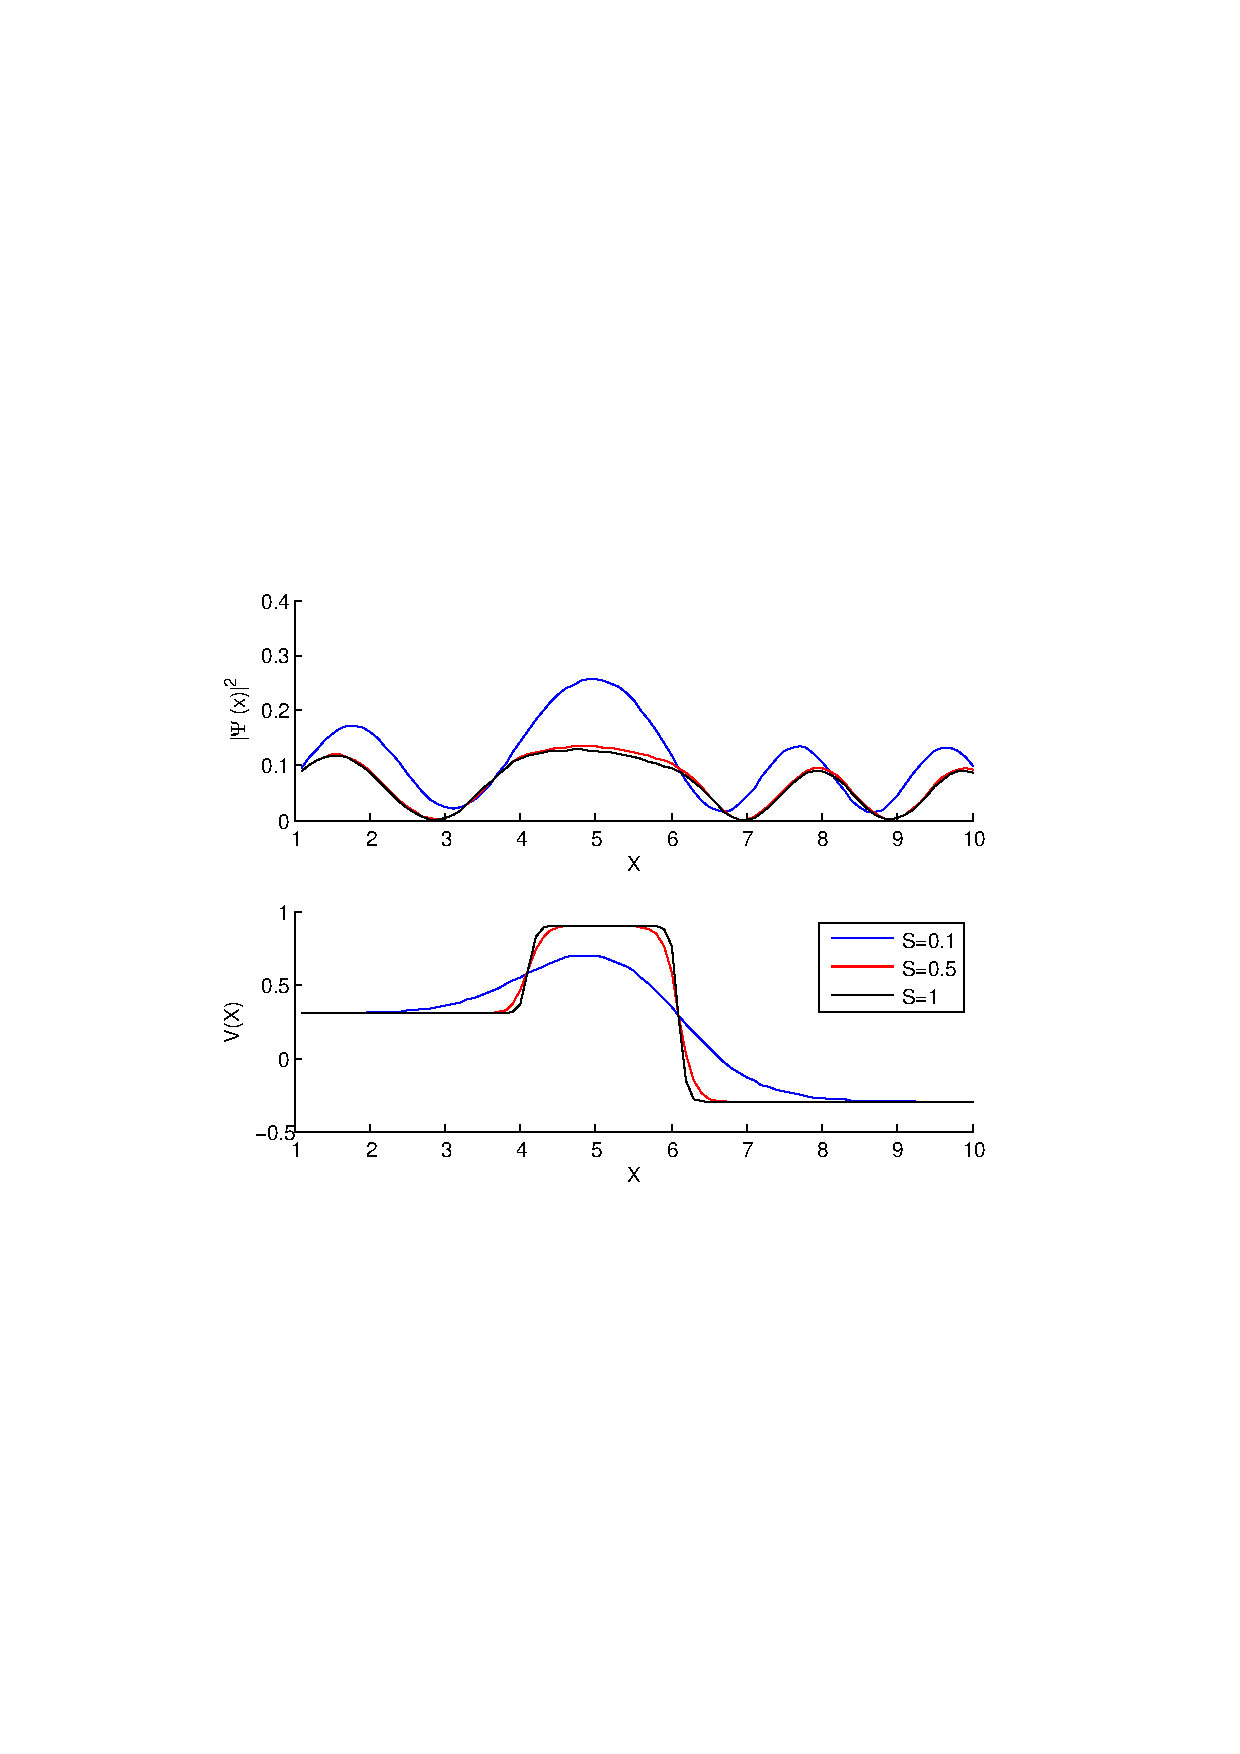
\includegraphics[scale=0.4, trim = 0mm 20mm 0mm 60mm, clip]{test2}
\label{fig:test2}
\end{figure}
\end{frame}

\begin{frame}
\begin{figure}
\centering
\caption{Amplitudes of wave-functions (upper graph) and potential barriers (lower graph) for the case: E=1.5, passing over the barrier, $\beta=0.5$, $x_1=4$, $x_2=6$, $V_{sd}=V_g=0.3$}
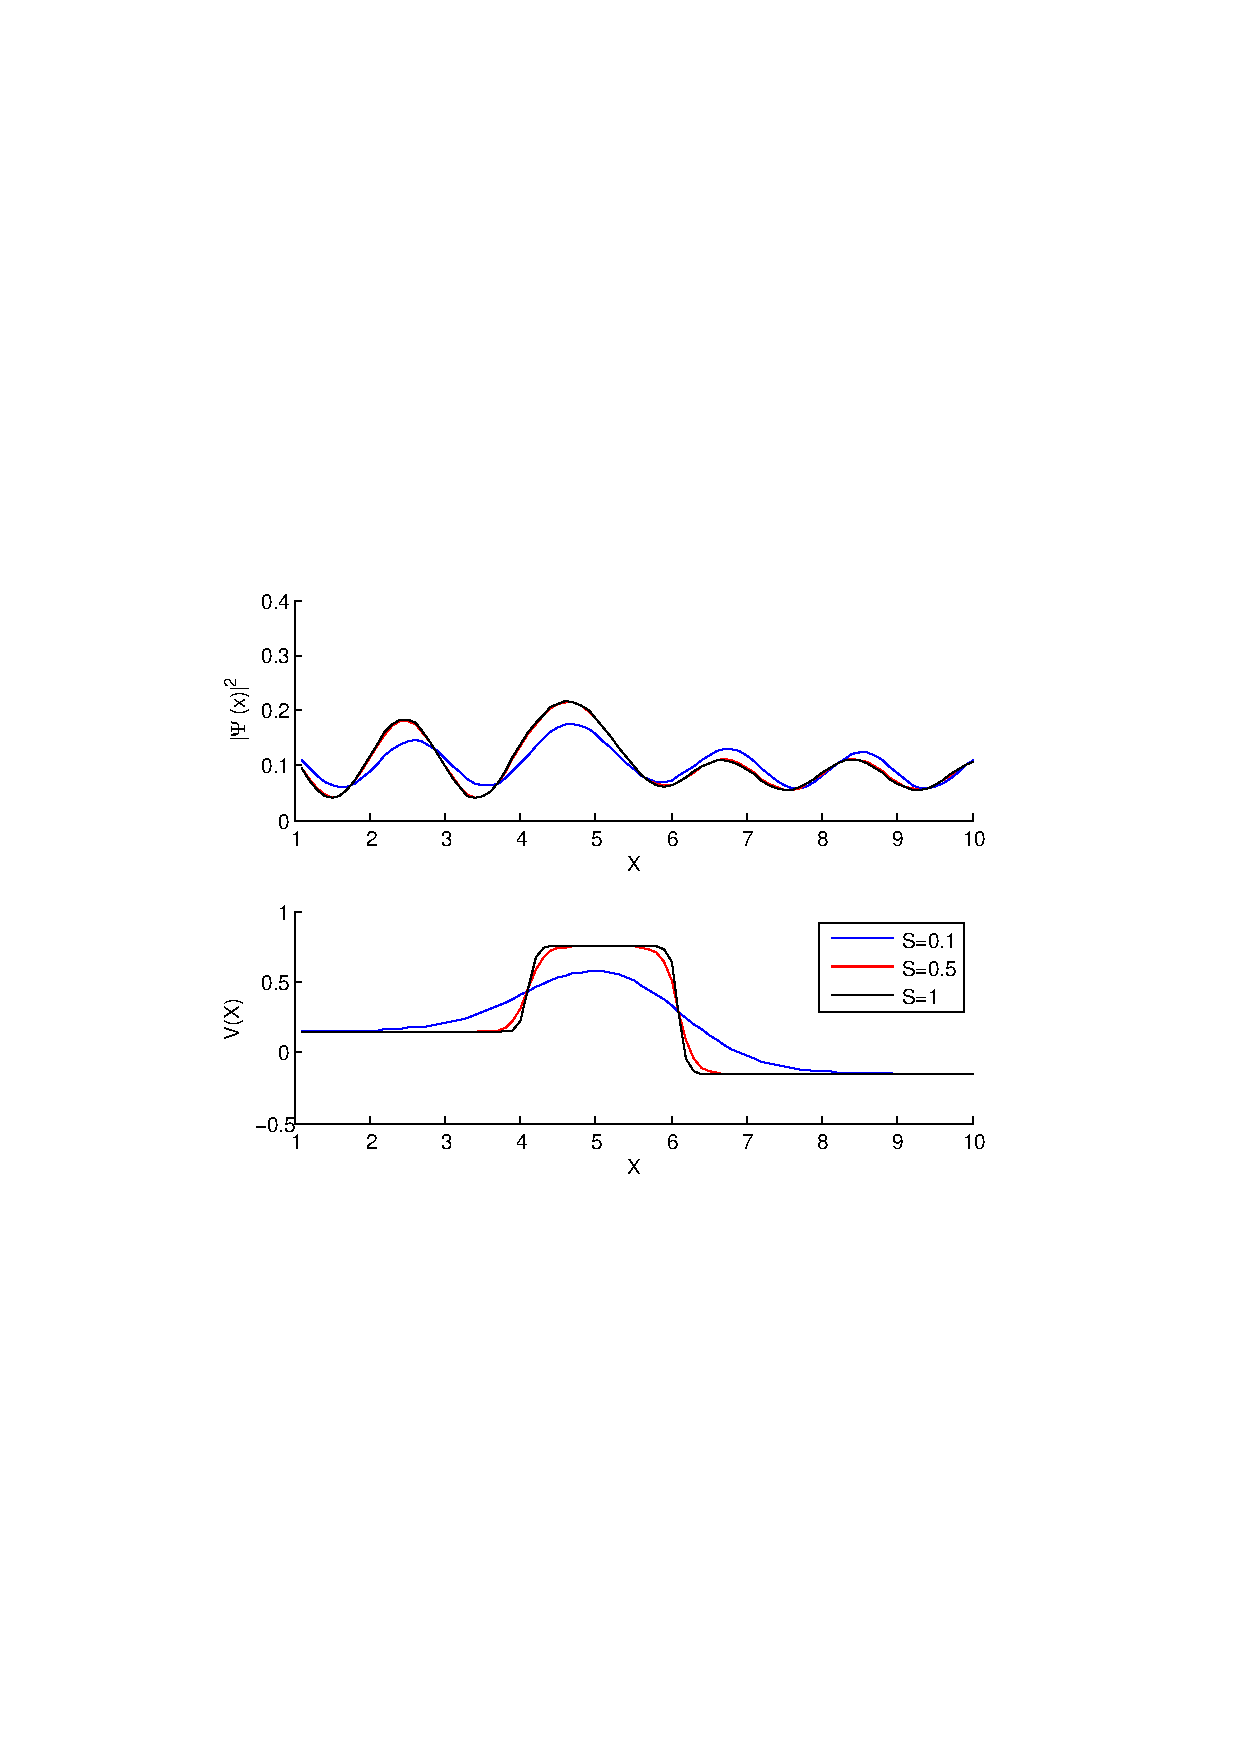
\includegraphics[scale=0.4, trim = 0mm 20mm 0mm 60mm, clip]{test3}
\label{fig:test3}
\end{figure}
\end{frame}

\section{Conclusion}
\begin{frame}
\begin{block}

We produced a solver that plotted the wavefunction and calculated transmition and reflection coefficients.
\end{block}
\end{frame}


\end{document} 